\documentclass[runningheads]{llncs}

\usepackage{graphicx}
\graphicspath{{figures/}}

\usepackage{amsmath}    % aligned equations
\usepackage{textcomp}   % beautiful teletype fonts and \textnumero
\usepackage{stmaryrd}   % short arrows
\usepackage[gen]{eurosym}
\usepackage{array}
\usepackage{booktabs} % nicer horizontal lines in tables
\usepackage{url}
\urlstyle{same}
\usepackage{microtype}
\usepackage[misc,geometry]{ifsym}

\usepackage{listings} % code listings
\lstdefinelanguage{Clean}{
	alsoletter={ABCDEFGHIJKLMNOPQRSTUVWXYZabcdefghijklmnopqrstuvwxyz_`1234567890},
	alsoletter={~!@\#$\%^\&*-+=?<>:|\\},
	alsoother={.},
	alsodigit={1234567890},
	morekeywords={generic,implementation,definition,dynamic,module,import,where,in,of,case,let,infix,infixr,infixl,class,instance,with,if,derive},
	sensitive=true,
	morecomment=[l]{//},
	morecomment=[n]{/*}{*/},
	morestring=[b]", % chktex 18
	morestring=[b]',
	emptylines=1,
	literate=   %
		% Basic Clean constructs
		{\\}{{$\lambda\:$}}1
		{\\n}{{\texttt{\textbackslash{}n}}}2
		{A.}{{$\forall\;\,$}}2
		{E.}{{$\exists\;\,$}}2
		%                {>}{{$>$}}1
		%                {<}{{$<$}}1
		{<=}{{$\leq$}}1
		{<=.}{{\texttt{<=.}}}3
		{>=}{{$\geq$}}1
		{<>}{{$\neq$}}1
		{->}{{$\shortrightarrow$}}2
		{<-}{{$\shortleftarrow$}}1
		{=}{{$=$}}1
		{~}{{$\sim$}}1
		% {\#}{{$\sharp$}}1
		{\{|}{{$\{\!|$}}2
		{|\}}{{$|\!\}$}}2
		{:=}{{$:=$}}2
		{==}{{\tiny{$==$}}}2
		{===}{{\tiny{$===$}}}3
		{++}{{\tiny$+\!\!+$}}2
		{+++}{{\tiny$+\!\!+\!\!+$}}3
		%                {+++}{{\tiny$+\!\!\!\!+\!\!\!\!+$}}3
		{:==}{{$:==$}}3
		{\{|*|\}}{{$\{\!|\!\star\!|\!\}$}}4
		%
		{<$>}{{\texttt{<\$>}}}3
		{<*>}{{\texttt{<*>}}}3
		{<|>}{{\texttt{<|>}}}3
		%
		% Basic iTask constructs
		{>||>}{{$\triangleright\triangleright$}}2
		%                {>>=}{{$>\!>=$}}3
		%                {>>|}{{$>\!>|$}3
		{>>>=}{{$>\!\!>\!\!>\!=$}}4
		{>>>|}{{$>\!\!>\!\!>\!|$}}4
		%                {>>>}{{$>\!>\!>$}}4
		{>>=}{{$>\!\!>\!=$}}3
		{>>|}{{$>\!\!>\!\!|$}}3
		{?>>}{{\texttt{?>\!>}}}3
		{!>>}{{\texttt{!>\!>}}}3
		{@>>}{{\texttt{@>\!>}}}3
		{<<@}{{\texttt{<\!<@}}}3
		{-||-}{{\texttt{-\!|\!\!|\!-}}}3
		{-||}{{\texttt{-\!|\!\!|}}}3
		{||-}{{\texttt{|\!\!|\!-}}}3
		{.||.}{{\texttt{.\!|\!\!|\!.}}}3
		{.&&.}{{\texttt{.\&\&.}}}4
}
\newcommand{\CleanInline}[1]{\lstinline[language=Clean]!#1!}
\newcommand{\prog}[1]{\CleanInline{#1}}
\lstdefinestyle{numbers}{numbers=left, stepnumber=1, numberstyle=\tiny, numbersep=5pt}
\lstnewenvironment{CleanCode}{\lstset{language=Clean}}{}
\lstnewenvironment{CleanCodeN}{\lstset{language=Clean,style=numbers}}{}
\makeatletter
\lst@AddToHook{OnEmptyLine}{\vspace{-0.5\baselineskip}}
\makeatother
\lstset{%
	captionpos=b,
	numberbychapter=false,
	breakatwhitespace=false,
	breaklines=true,
	keepspaces=true,
	basicstyle=\linespread{0.9}\small\tt,
	identifierstyle=\footnotesize\tt,
	commentstyle=\normalfont\it,
	keywordstyle=\footnotesize\bf,
	showspaces=false,
	showstringspaces=false,
	showtabs=false,
	tabsize=4,
	basewidth=0.43em,
	columns=[c]fixed,
	texcl=true,
	numbers=none,
	showstringspaces=false,
	keepspaces=true,
	breaklines=false,
	escapeinside={(\#}{\#)}, %chktex 9
}

\hyphenation{%
	pa-ra-digm
	func-tio-nal
	re-ac-ti-ve
	pro-gram-ming
}

\begin{document}
%
\title{Reducing the Power Consumption of IoT with Task-Oriented Programming}
%
%\titlerunning{Abbreviated paper title}
% If the paper title is too long for the running head, you can set
% an abbreviated paper title here
%
\author{%
	Sjoerd~Crooijmans \and % chktex 8
	Mart~Lubbers\textsuperscript{\Letter}\orcidID{0000-0002-4015-4878} \and % chktex 8
	Pieter~Koopman\orcidID{0000-0002-3688-0957} % chktex 8
}
%
\authorrunning{S.\ Crooijmans et al.}
% First names are abbreviated in the running head.
% If there are more than two authors, 'et al.' is used.
%
\institute{Institute for Computing and Information Sciences, Radboud University Nijmegen, The Netherlands\\
\email{sjoerd@scrooijmans.nl}
\email{\{mart,pieter\}@cs.ru.nl}}
%
\maketitle              % typeset the header of the contribution
%

\begin{abstract}
	Limiting the energy consumption of IoT nodes is a hot topic in green computing. For battery-powered devices this necessity is obvious, but the enormous growth of the number of IoT nodes makes energy efficiency important for every node in the IoT.
	In this paper, we show how we can automatically compute execution intervals for our task-oriented programs for the IoT.
	These intervals offer the possibility to save energy by bringing the microprocessor driving the IoT node into a low-power sleep mode until the task need to be executed.
	Furthermore, they offer an elegant way to add interrupts to the system.
	We do allow an arbitrary number of tasks on the IoT nodes and achieve significant reductions of the energy consumption by bringing the microprocessor in sleep mode as much as possible.
	We have seen energy reductions of an order of magnitude without imposing any constraints on the tasks to be executed on the IoT nodes.
%\mlcomment{Moet hier niet nog vernoemd worden dat we ook interrupts hebben toegevoegd?}
%\pkcomment{Goede. Gedaan}.

	\keywords{Sustainable IoT  \and Green Computing \and Task-Oriented Programming \and Edge computing.}
\end{abstract}
%
\section{Introduction}
The Internet of Things (IoT) is omnipresent and powered by software.
Depending on whom you ask, the estimated number of connected IoT devices reached between 25 and 100 billion in 2021.
IoT systems are traditionally designed according to multi-layered or tiered architectures.
As a consequence, discrete programs written in distinct languages with different abstraction levels power the individual layers, forming a heterogeneous system.
%For example, the web interface may be using javascript while the server is a java application, a SQL database stores the data, MQTT over Bluetooth low energy is used for the communication and the microprocessors in the edge layer are programming in the low-level C language.
%This heterogeneity also occurs within the device or edge layer, where there is a great variety of microprocessors each with its architectures, frameworks and power modes.
The variation in components makes programming IoT systems complicated, error-prone and expensive.
%\pkcomment{kunnen al die talen niet later of weg? Ze zijn niet erg essentieel voor dit paper.}

The edge layer of IoT contains the small devices that sense and interact with the world and it is crucial to lower their energy consumption.
While individual devices consume little energy, the sheer number of devices in total amounts to a lot.
Furthermore, many IoT devices operate on batteries and higher energy consumption increases the amount of e-waste as IoT devices are often hard to reach and consequently hard to replace~\cite{NIZETIC2020122877}.

To reduce the power consumption of an IoT device, the specialized low-power sleep modes of the microprocessors can be leveraged.
Different sleep modes achieve different power reductions because of their different run time characteristics.
These specifics range from disabling or suspending Wi-Fi; stopping powering (parts) of the {RAM}; disabling peripherals; or even turning off the processor completely, requiring an external signal to wake up again.
Determining when exactly and for how long it is possible to sleep is expensive in the general case and often requires annotations in the source code, a real-time operating system or a handcrafted scheduler.

Task-oriented programming (TOP) is a novel declarative programming paradigm with the potential to solve many of the aforementioned problems.
In this paradigm, tasks are the basic building blocks and they can be combined using combinators to describe workflows~\cite{plasmeijer_task-oriented_2012}.
This declarative specification of the program only describes the \emph{what} and not the \emph{how} of execution.
The system executing the tasks takes care of the gritty details such as the user interface, data storage and communication~\cite{frp_vs_top}.
An example of a TOP language is the iTask system, a general-purpose framework for specifying multi-user distributed web applications for workflows~\cite{TOP-ICFP07}.
iTask is implemented as an embedded domain-specific language (DSL) in the functional programming language Clean~\cite{brus_clean_1987,Clean:language}.
%Generics~\cite{GenericProgrammingExtensionForClean,HinzeGenericFunctionalProgramming} are used to derive default versions of required manipulations of datatypes.

mTask lies on the other side of the spectrum and aims to solve semantic friction in IoT.
It is a domain-specific TOP language and system specifically designed for IoT devices, implemented as an embedded DSL in iTask.
Where iTask abstracts away from details such as user interfaces, data storage, and persistent workflows, mTask offers abstractions for edge layer-specific details such as the heterogeneity of architectures, platforms and frameworks; peripheral access; and multitasking.
Yet, it lacks abstractions for energy consumption and scheduling.
In mTask, tasks are implemented as a rewrite system, where the work is automatically segmented in small atomic bits and stored as a task tree.
Each cycle, a single rewrite step is performed on all task trees, during rewriting, tasks do a bit of their work and progress steadily, allowing interleaved and seemingly parallel operation.
After a loop, the run-time system (RTS) knows which task is waiting on which triggers and is thus able to determine the next execution time for each task automatically.
Utilising this information, the RTS can determine when it is possible and safe to sleep and choose the optimal sleep mode according to the sleeping time.
For example, the RTS never attempts to sleep during an I$^2$C communication because I/O is always contained \emph{within} a rewrite step.

%\pkcomment{Is het nodig om hier over itasks te praten?}
%\pkcomment{Kunnen we niet benadrukken dat TOP een prima basis geeft om te bepalen wanneer (b.v. alle IO binnen een rewrite step) er geslapen kan worden en hoelang?}

%Paragraph 2: What is TOP/mTask?
%\begin{itemize}
%	\item TOP is a new programming paradigm.
%	\item Tasks are the basic building blocks
%	\item Tasks can be combined with combinators
%	\item Abstractions are available for details such as communication, user interfaces, data storage.
%	\item mTask is a TOP implementation for IoT devices integrated into iTask, a general-purpose TOP framework for distributed multi-user workflow applications.
%	\item mTask offers abstractions for IoT specific details such as peripheral access, multi-tasking network but no energy consumption/scheduling.
%\end{itemize}

\subsection{Research contribution}
This paper shows that with minor changes to the mTask language from the perspective of the TOP programmer, the energy consumption of the program's execution can be significantly reduced.
We show that with an intensional analysis of the task trees at run time, the mTask scheduler can automatically determine the optimal sleep time and sleep mode.
Not all tasks have a default rewrite rate that works in all situations, so variants of tasks are added in which the programmer can fine-tune the polling rate.
Furthermore, we add an interface to (hardware) interrupts to the mTask language, allowing the program to be notified in case of an external event, resulting in more reactive programs.

%Paragraph n: Research contribution
%\begin{itemize}
%	\item Peripheral tasks can be finetuned for polling rate
%	\item Interrupt tasks can be defined
%	\item The mTask RTS implements a scheduler that automatically sleeps for as long as possible
%\end{itemize}

\section{Task-Oriented Programming}%
\label{sec:top}

TOP is a high-level declarative programming paradigm to specify distributed interactive multi-user systems~\cite{TOP-ICFP07,plasmeijer_task-oriented_2012}.
Developers describe in TOP the work to be done by the systems or users in the form of abstract tasks.
Implementation details, like the encoding of data %\mlcomment{snap ik niet}
during communication, are handled by the system rather than by the TOP programmer. %\pkcomment{beter?} Mart: Ja
Tasks describe a unit of work ranging from reading a single sensor to an entire IoT system.
Tasks are rewrite systems that produce a result after each step. Possible task results are:
\begin{description}
\item[No value] if the task has no observable value for other tasks.
For example, a web-editor that is empty or incomplete is a task with a \prog{NoValue} result.
\item[Unstable] if the task has an intermediate observable value.
This value is by construction properly typed and can change in the future.
Examples are a properly filled out web-editor or a reading a sensor.
\item[Stable] if the task has a final observable value.
This value is by construction properly typed and fixed.
Examples are a properly filled out web-editor after pressing the \prog{Continue} button or a task that determines that a temperature sensor has passed a given threshold.
\end{description}

Basic tasks are the primitive building blocks of a TOP program.
Typical examples are web-editors, reading sensors, waiting some time and controlling peripherals.
Tasks can be composed into bigger tasks by combinators.
There are combinators for the parallel and sequential composition of tasks.
%The \emph{step} combinator is used to specify actions, selecting a new task, based on the current value of some task.\mlcomment{Is deze informatie nodig?}

Apart from task results, tasks can also communicate via shared data sources (SDSs).
There are basic tasks to read, write and update such a typed {SDS}.

%Stukje over tierless system

% We illustrate some of the possibilities with the example in Listing~\ref{lst:plants}.
% This makes an editor for a list of plants.
% A \prog{Plant} is a record with a \prog{species} of type String and a \prog{location} of the enumeration type \prog{Location}.
% The \prog{derive} generates all required machinery to handle the types \prog{Plant} and \prog{Locantion} in iTasks.
% The \prog{enterPlants} function is a task that yields a list of plants.
% The combinator \prog{>>!} generates the continue button, it is enables whenever the editor on the left-hand side has a value.
% \begin{lstlisting}[language=Clean,caption={An iTask web-editor for Plants},label={lst:plants}]
% import iTasks

% :: Location = LivingRoom | Kitchen | Garden | Greenhouse
% :: Plant = { species :: String, location :: Location }

% derive class iTask Location, Plant

% enterPlants :: Task [Plant]
% enterPlants = enterInformation [] >>! return

% Start world = doTasks enterPlants world
% \end{lstlisting}
% This program generates a webserver that generates here a web-editor for a list of plants.
% In Figure~\ref{fig:plants} we display two screenshots of this editor.
% On the left the editor has no value since there is no proper \prog{species} specified.
% On the right the list contains two proper plants and the \prog{Continue} button is enabled.
% Pressing this button would produce the list of these two plants as a stable value.
% \begin{figure}[htb]
% 	\begin{minipage}{.49\linewidth}
% 		\fbox{\includegraphics[width=.95\textwidth]{figures/plants0.jpg}}
% 	\end{minipage}%
% 	\begin{minipage}{.49\linewidth}
% 		\fbox{\includegraphics[width=.95\textwidth]{figures/plants.jpg}}
% 	\end{minipage}
% 	\caption{Screenshots of the enterPlants editor: NoValue (left) and Unstable (right).}%
% 	\label{fig:plants}
% \end{figure}
% Such an iTask program is efficient since only edit events causes a new evaluation of the task expression.
% When there are no edit events from the browser to handle, the webserver is waiting and consumes no energy.
% The operating system running the webserver takes care about the energy consumption of the machine running the webserver.
% The client interacting with humans is any browser running on some system that has an internet connection with the webserver.

\subsection{mTask}%
\label{sec:mtask}

TOP is also very suited to program nodes in the IoT.
However, typical nodes in the IoT are cheap and small microprocessors with a very limited amount of processing power and memory.
Such a system cannot run a web server nor a browser as a client to execute an iTask program.
This is also not necessary, typical IoT nodes just control a few sensors and actuators.
Rather than sending all sensor readings to some server and the actuator control back from the server to the IoT node, we want to do a significant part of the computing on the IoT nodes.
This concept is popular under the name edge computing.

To enable TOP on small microprocessors we have created mTask~\cite{koopman_task-based_2018,lubbers20tiered}.
The domain-specific language mTask is also embedded in Clean.
In contrast to iTask, it is not a shallowly embedded DSL but it is a tagless-final style DSL~\cite{FinallyTagless}.
The target language of iTask is equal to the host language Clean, this is called a homogeneous DSL~\cite{TrattDSL}.
The target code of mTask is byte code which is shipped to a microprocessor in the IoT and interpreted by the mTask runtime system running there.
Hence, mTask is a heterogeneous embedded {DSL}.
The big advantage of this approach is that we can carefully control which parts of the application is mTask code and needs to be shipped to the IoT node.
This prevents that all Clean language machinery ends up in such a small system.
Moreover, we can dynamically ship tasks to the IoT nodes without the need to reprogram the flash memory of those systems.
Reprogramming this memory is slow and can be done only a few thousand times.

The archetypal example of programs running on microprocessors is the blink example that blinks the single bit \emph{display}, just a LED, of such systems.
In Listing~\ref{lst:blink} we give a slightly more complex example in mTask that blinks two LEDs at their own slowly changing speed.

\begin{lstlisting}[language=Clean,caption={An mTask task to blink two LEDs at their own rate.},label={lst:blink}]
blinkTask :: Main (MTask v Bool) | mtask v
blinkTask = declarePin BuiltinLEDPin PMOutput \led1 ->
            declarePin D0 PMOutput \led2 ->
            fun \blink = (\(led, interval, state) ->
                     delay interval
                >>|. writeD led state
                >>|. blink (led, interval +. lit 1, Not state)
            In {main = blink (led1, lit 496, true) .||. blink (led2, lit 8128, true)}
\end{lstlisting}

The Clean function \prog{blinkTask} contains the mTask code for the blink task.
It starts by declaring two \prog{led} objects to represent the output general-purpose input/output pin to control the LED as output.
Next, it declares an mTask function called \prog{blink}.
This function has the \prog{led}, delay \prog{time} and new \prog{state} of the LED as arguments.
The task in this function is composed of three subtasks.
First, it waits \prog{time} millisecond by \prog{delay}.
Second, it writes the given \prog{state} to the declared output \prog{led}.
Finally, it calls itself recursively with the inverted \prog{state} as the argument.
In the \prog{main} expression two of these \prog{blink} tasks are composed in parallel with the \prog{.||.} combinator.
The \prog{lit} in the arguments of the subtasks lifts the given constant from the host language to the embedded {DSL}.

There are some important differences to the usual C-programs controlling microprocessors.
First, tail-recursive functions are perfectly safe in mTask.
Next, the \prog{delay} task is not blocking the entire program, but just producing a \prog{NoValue} result until the given \prog{time} has passed.

\section{Energy Efficient IoT Nodes}

There are various estimates about the number of IoT nodes.
What the estimates have in common is that the number is relatively large and rapidly increasing.
Figure~\ref{fig:iotNodes} contains a popular estimate of the worldwide number of nodes%
\footnote{\url{https://statinvestor.com/data/33967/iot-number-of-connected-devices-worldwide/}}.
Currently, there are worldwide just above 40 billion connected IoT devices.

\begin{figure}[ht]
	\centering
	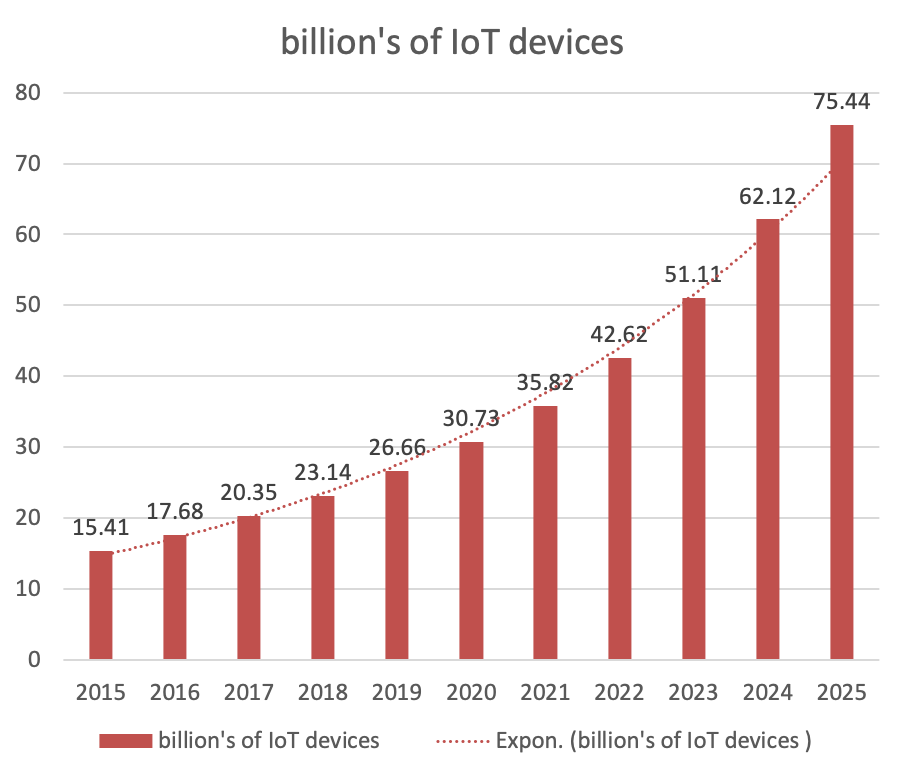
\includegraphics[width=.6\linewidth]{iotNodes}
	\caption{Number of connected IoT nodes worldwide.}%
	\label{fig:iotNodes}
%	\vspace{-.5cm}
\end{figure}

There is a wide variety of IoT nodes.
Relative simple single board computers, like a Raspberry Pi 4, are often used.
These are full-fledged computers running Linux.
This operating system enables multithreading and the dynamic uploading of new applications via remote access.
Such a single board computer costs about \euro{70} and consumes 4--6W.

For battery powered nodes, the energy consumption of such a single board computer is obviously inconveniently high.
Considering the number of IoT nodes, the total energy consumption for all nodes would also be rather high for single board computers connected to a power outlet.
The total annual energy consumption of all IoT nodes would be 1.7 PWh/year if they consume 5W each and are always available.
This is about $6\%$ of the annual electrical energy production of 26.8 PWh/year%
\footnote{\url{https://www.bp.com/en/global/corporate/energy-economics/statistical-review-of-world-energy/electricity.html}}, about 500 times the production of the only Dutch nuclear power plant%
\footnote{\url{https://nl.wikipedia.org/wiki/Kerncentrale_Borssele}},
and $\frac{2}{3}$ of the annual production of renewable electricity\footnotemark{}.
\footnotetext{\url{https://www.bp.com/content/dam/bp/business-sites/en/global/corporate/pdfs/energy-economics/statistical-review/bp-stats-review-2021-electricity.pdf}}

Fortunately, there are microprocessor based systems that require significantly less energy, typically 1--500 mW, than single board computers and are very cheap as well.
The price to be paid is that microprocessors are much slower and have a very limited amount of memory.
As a consequence of these bordered capacities, a microprocessor typically has no operating system or at most special purpose real-time operating system like {FreeRTOS}.
Despite their limited capabilities, microprocessors are often more powerful than needed for IoT tasks.
This implies that we can switch them off, or partially off, for some fraction of the time.
Microprocessors have special low power sleep modes to enable energy saving.
The sleep modes as well as the associated energy consumption are model specific.
Table~\ref{tbl:sleep} lists some examples for two popular microprocessor boards.
The Wemos D1 mini%
\footnote{\url{https://www.wemos.cc/en/latest/d1/d1_mini.html}}
is powered by an ESP8266 and costs about \euro{6}.
The Adafruit Feather M0 WiFi%
\footnote{\url{https://www.adafruit.com/product/3010}}
is powered by an ATSAMD21 and an ATWINC1500 for Wi-Fi, it costs about \euro{50}.

\begin{table}[t]
	\centering
	\begin{tabular}{ccccccccc}
		\toprule
		& \multicolumn{4}{c}{Wemos D1 mini} & \multicolumn{4}{c}{Adafruit Feather M0 Wifi} \\
		\midrule
		component & active & modem & light & deep & active & modem & light & deep \\
				  & & sleep & sleep & sleep & & sleep & sleep & sleep \\
				  \midrule
		Wi-Fi & on & off & off & off  & on & off & off & off \\
		CPU & on & on & pending & off & on & on & idle & idle \\
		RAM & on & on & on & off & on & on & on & low power \\
		current & 100--240 & 15 & 0.5 & 0.002 & 90--300 & 5 & 2 &  0.005\\
		\bottomrule
	\end{tabular}
	%\vspace{0.25cm}
	\caption{Current use in mA of two microprocessor boards in various sleep modes.}%
	\label{tbl:sleep}
	%\vspace{-0.5cm}
\end{table}
%\mlcomment{Ik vind de tabel zo een stuk mooier (en de algemene drukkerij community ook). Verticale strepen zijn meestal een doodzonde}
%\pkcomment{Prima. Alleen de ``power'' van ``Low power'' is een beetje raar. In de zin van niet erg duidelijk waar die bij hoort.}
%\mlcomment{beter?}
%\pkcomment{top}

This table shows that switching the Wi-Fi radio off yields the biggest energy savings.
In most IoT applications, we need Wi-Fi for communications.
It is fine to switch it off, but after switching it on, the Wi-Fi protocol needs to transmit a number of messages to re-establish the connection.
This implies that it is only worthwhile to switch the radio off when this can be done for some time.
The details vary per system and situation.
As a rule of thumb, it is only worthwhile to switch the Wi-Fi off when it is not needed for at least some tens of seconds.

The data in Table~\ref{tbl:sleep} shows that it is worthwhile to put the system in some sleep mode when there is temporarily no work to be done.
A deeper sleep mode saves more energy, but also requires more work to restore the software to its working state.
A processor like the ESP8266 driving the Wemos D1 mini loses the content of its RAM in deep sleep mode.
This implies that the program itself is preserved, since it is stored in flash memory, but the entire program state is lost.
When there is a program state to be preserved, we must either store it elsewhere, limit us to light sleep, or use a microprocessor that keeps the RAM intact during deep sleep.

For IoT nodes executing a single task, explicit sleeping to save energy can be achieved without too much hassle.
This becomes much more challenging as soon as multiple independent tasks run on the same node.
Sleeping of the entire node induced by one task prevents progress of all tasks.
This is especially annoying when the other tasks are executing time critical parts, like communication protocols.
Such protocols control the communication with sensors and actuators.
Without the help of an OS, the programmer is forced to combine all subtasks into one big system that decides if it is safe to sleep for all subtasks.

\section{Scheduling Tasks Efficiently}%
\label{sec:SchedulingTasksEfficiently}

The mTask system enables an elegant solution for these dynamic scheduling and sleeping problems.
To understand the solution, we have to reveal some details about the mTask implementation.
This system consists of two components.
First, there is the embedded DSL as introduced in Section~\ref{sec:mtask}.
Next, there is an execution environment for those programs running on IoT nodes.
This execution environment is able to execute multiple mTask programs simultaneously, it is a featherlight domain-specific operating system.
%originating potentially from different sources
%\mlcomment{Ik snap niet goed wat je hier mee bedoelt. Een mTask client kan niet met meerdere servers tegelijkertijd praten. Het kan wel meerdere taken tegelijkertijd uitvoeren}, 


Every mTask program is embedded in an iTask program, a TOP DSL very similar to mTask.
In contrast to mTask, iTask is geared to client server web-applications.
The iTask and mTask components form a single source that is statically type-checked by the compiler of the host language Clean.
The mTask components determine what is done by the IoT nodes.
The surrounding iTask program determines the IoT node to be used and the moment it is shipped.
The communication between iTask and mTask programs is outside the scope of this paper, see~\cite{lubbers_writing_2019} for details.

A mTask program is dynamically transformed to byte code.
This byte code and the initial mTask expression are shipped to mTask IoT node.
For the example in Listing~\ref{lst:blink} there is byte code representing the \prog{blink} function and \prog{main} determines the initial expression.

The mTask rewrite engine rewrites the current expression just a single rewrite step at a time.
When subtasks are composed in parallel, like blink tasks in Listing~\ref{lst:blink}, all subtasks are rewritten unless the result of the first rewrite step makes the result of the other tasks superfluous.
This yields for our example:

\begin{lstlisting}[language=Clean,caption={State of the task from Listing~\ref{lst:blink} after a single rewrite step.},label={lst:blink-step}]
{main =  delay 496  >>|. writeD led1 true >>|. blink (led1, 497, false)
     .||. delay 8128 >>|. writeD led2 true >>|. blink (led2, 8129, false)}
\end{lstlisting}

The mTask node can inspect this expression.
It is obvious that nothing will change the next 496ms.
The system can therefore go to sleep for this period when there are no other tasks\footnotemark{}.
\footnotetext{In the implementation a \prog{delay d} is replaced by a \prog{waitUntil (now + d)} that compares the clock time of the system with the given start time.}

The task design ensures such that all time critical communication with peripherals is within a single rewrite step.
This is very convenient, since the system can inspect the current state of all mTask expressions after a rewrite and decide if sleeping and how long is possible.
%As a consequence, we cannot have fair preemptive multitasking.
As a consequence, we cannot have fair multitasking.
%\todo[author={reviewer 2}]{Page 7: I'm not clear on why fair multitasking isn't allowed. Would it
%be more correct to say it isn't ``supported'', or is there something
%about the mTask evaluation model that fundamentally prohibits
%concurrent evaluation?}
%\mlcomment{Dit zouden we moeten uitleggen: We kunnen we preemptive multitasking, maar het is moeilijk en duur dat automatisch te doen omdat je I/O hebt e.d.}
When a single rewrite step would take forever due to an infinite sequence of function calls, this would block the entire IoT node.
Infinite sequences rewrite steps, as in the \prog{blink} example above, are perfectly fine.
The mTask system does proper tail-call optimizations to facilitate this.


% In each rewrite, all leaves of the task expression are evaluated.
% Whenever enabled by the current value of its arguments an mTask combinator evaluates to its results.
% When a reduction is not yet possible the mTask expression is recreated with the new arguments.
% This explains for instance why the \prog{delay} in Listing~\ref{lst:blink} is not blocking.
% This is very similar to the implementation of iTask.
% In iTask, the task expression is evaluated again at an event, like an edit event form a web-editor.
% In mTask, we do not have editor events.
% Most sensors work with polling rather than on an event basis.
% Hence, the mTask interpreter evaluates the task expression in a tight loop.
% Since no other programs are running on the microprocessor and its cycles have to be used by executing some instructions, such a frequent evaluation of the task expression is perfectly fine.

% Microprocessors offer various ways to reduce their power consumption.
% These range from switching off parts of the system that are temporarily not needed, such as the Wi-Fi radio, to putting the entire system into some sleep mode.
% Different branches of microprocessors offer diverse sleeping modes.
% In this paper, we will distinguish light sleep where the memory stays powered and hence its contents will be unaffected by sleeping and deep sleep where also the memory is switched off and its content will be lost.
% Some microprocessors have parts of the memory that will be saved in deep sleep. Since that is very brand specific we will ignore that here.

% In this paper, we introduce a way to reduce the power consumption of a microprocessor implementing mTask by sleeping as much as possible.
% When there is no mTask to be executed the system goes to deep sleep mode. It just wakes up every now and then to keep the Wi-Fi connection active and checks for a new mTask to be executed.
% When there are one or more mTasks to be executed it tries to predict when it is useful to evaluate the mTask expression again.
% For instance, evaluating a \prog{delay(time)} expression can be delayed \prog{time} milliseconds without a problem. No progress will be made before the delay time has passed.
% Also for many sensors, it is possible to reduce the evaluation rate.
% In most applications, a temperature measured by a sensor will not change significantly within a couple of seconds.
% We can safely delay the reading of such a sensor.


\subsection{Evaluation Interval}

Some mTask examples contain one or more explicit \prog{delay} primitives, offering a natural place for the node executing it to pause.
However, there are many mTask programs that just specify a repeated set of primitives.
A typical example is the program that reads the temperature for a sensor and sets the system LED if the reading is below some given \prog{goal}.

\begin{lstlisting}[language=Clean,caption={A basic thermostat task.},label={lst:thermostat}]
thermostat :: Main (MTask v Bool) | mtask v
thermostat = DHT I2Caddr \dht.
             {main = rpeat (
                 temperature dht >>~. \temp.
                 writeD builtInLED (goal <. temp)
             )}
\end{lstlisting}

This program repeatedly reads the DHT sensor and sets the on-board LED based on the comparison with the \prog{goal} as fast as possible on the mTask node.
This is a perfect solution as long as we ignore the power consumption.
The mTask machinery ensures that if there are other tasks running on the node, they will make progress.
However, this solution is far from perfect when we take power consumption into account.
In most applications, it is very unlikely that the temperature will change significantly within one minute, let alone within some milliseconds.
Hence, it is sufficient to repeat the measurement with an appropriate interval.

There are various ways to improve this program.
The simplest solution is to add an explicit delay to the body of the repeat loop, similar to the blink example in Listing~\ref{lst:blink}.
A slightly more sophisticated option is to add a repetition period to the \prog{rpeat} combinator.
The combinator implementing this is called \prog{rpeatEvery}.
Both solutions rely on an explicit action of the programmer.

In this paper, we propose a solution that is independent of the help of the programmer.
The key of this solution is to associate dynamically an evaluation interval with each task.
The interval $\langle {low}, {high} \rangle$ indicates that the evaluation can be safely delayed by any number of milliseconds in that range.
Such an interval is just a hint for the run time system.
It is not a guarantee that the evaluation takes place in the given interval.
Other parts of the task expression can force an earlier evaluation of this part of the task.
When the system is very busy with other work, the task might even be executed after the upper bound of the interval.
The system calculates the refresh rates from the current task expression.
This has the advantage that the programmer does not have to deal with them and that they are available in each and every mTask program.

\subsection{Basic Refresh Rates}

We start by assigning default refresh rates to basic tasks.
These refresh rates reflect the expected change rates of sensors and other inputs.
Writing to basic GPIO pins and actuators has refresh rate $\langle 0, 0 \rangle$, this is never delayed.

\begin{table}
	\centering
	\begin{tabular}{ll}
		\toprule
		task & default interval \\
		\midrule
		reading an SDS & $\langle 0, 2000 \rangle$ \\
		slow sensor, like temperature & $\langle 0, 2000 \rangle$ \\
		gesture sensor & $\langle 0, 1000 \rangle$ \\
		fast sensor, like sound or light & $\langle 0, 100 \rangle$ \\
		reading GPIO pins & $\langle 0, 100 \rangle$ \\
		\bottomrule
	\end{tabular}
	\caption{Default refresh rates of basic tasks.}%
	\label{tab:refresh}
	%\vspace{-1.5cm}
\end{table}

% The \prog{delay(time)} primitive guarantees that the task will be delayed at least \prog{time} milliseconds.
% Since mTask is not a hard real-time system also this delay might be higher than the given time since the microprocessor might be busy with other things, like handling Wi-Fi communication.

\subsection{Deriving Refresh Rates}

Based on these refresh rates, the system can automatically derive refresh rates for composed mTask expressions using $\mathcal{R}$.
We use the operator $\cap_{\textit{safe}}$ to compose refresh ranges.
When the ranges overlap the result is the overlapping range.
Otherwise, the result is the range with the lowest numbers.
The rationale is that subtasks should not be delayed longer than their refresh range.
Evaluating a task earlier should not change its result but can consume more energy.


\begin{align}
	\cap_{\textit{safe}} :: \langle \mathit{Int}, \mathit{Int} \rangle \; \langle \mathit{Int}, \mathit{Int} \rangle & \shortrightarrow \langle \mathit{Int}, \mathit{Int} \rangle & \notag \\
	R_1 \cap_{\textit{safe}} R_2 & = R_1 \cap R_2 & \text{if } R_1 \cap R_2 \neq \emptyset \\
	\langle l_1, h_1 \rangle \cap_{\textit{safe}} \langle l_2, h_2 \rangle & = \langle l_2, h_2 \rangle & \text{if } h_2 < l_1 \\
	R_1 \cap_{\textit{safe}} R_2 & = R_1  & \text{otherwise}
\end{align}

\begin{align}
	\mathcal{R} :: (\mathit{MTask}~v~a)    & \shortrightarrow \langle \mathit{Int}, \mathit{Int} \rangle \notag \\
	\mathcal{R} (t_1~{.||.}~t_2)  & = \mathcal{R}(t_1) \cap_{\textit{safe}} \mathcal{R}(t_2) \label{R:or} \\
	\mathcal{R}(t_1~{.\&\&.}~t_2) & = \mathcal{R}(t_1) \cap_{\textit{safe}} \mathcal{R}(t_2) \label{R:and}\\
	\mathcal{R}(t_1~{>\!\!>\!|.}~t_2)   & = \mathcal{R}(t_1) \label{R:seq} \\
	\mathcal{R}(t~{>\!\!>\!=.}~f)       & = \mathcal{R}(t) \label{R:bind} \\
	\mathcal{R}(t~{>\!\!>\!\!*.}~[a_1 \ldots a_n]) & = \mathcal{R}(t) \label{R:step} \\
	\mathcal{R}(\mathit{rpeat}~t)             & = \langle 0, 0 \rangle \label{R:rpeat} \\
	\mathcal{R}(\mathit{rpeatEvery}~d~t)   & = \langle 0, 0 \rangle \label{R:rpeatevery} \\
	\mathcal{R}(delay~d) & = \langle d, d \rangle \label{R:delay} \\
	\mathcal{R}(t) & =
		\left\{%
			\begin{array}{ll}
				\langle \infty, \infty \rangle~& \text{if}~t~\text{is Stable} \\
				\langle r_l, r_u \rangle & \text{otherwise}
			\end{array}
		\right.\label{R:other}
\end{align}

% \mathcal{R}(rpeatEvery \; d \; t)   & =
%     \left\{%
%         \begin{array}{ll}
%             \mathcal{R}(t) & \text{if} \; t \; \text{is UnStable} \\
%             \langle d, d \rangle \; & \text{otherwise}
%         \end{array}
%     \right.\label{R:rpeatevery} \\


We will briefly discuss the various cases of deriving refresh rates together with the task semantics of the different combinators

\subsubsection{Parallel Combinators} For the parallel composition of tasks we compute the intersection of the refresh intervals of the components as outlined in the definition of $\cap_{\textit{safe}}$.
The operator \prog{.||.} in Equation~\ref{R:or} is the \emph{or}-combinator; the first subtask that produces a stable value determines the result of the composition.
The operator \prog{.&&.} in Equation~\ref{R:and} is the \emph{and}-operator. The result is the tuple containing both results when both subtasks have a stable value.
%The refresh rates of the parallel combinators have no direct relation with their task result.
%\mlcomment{Dit is verwarrend, het ghaat toch om refresh rates en niet om task values? Misschien moeten we in dat zinnetje hierboven ook vermelden dat we een semantiek geven van de taakwaardes.}
%\pkcomment{Maar dit is de eerste keer dat \texttt{.\&\&.} langs komt, ik denk dat we iets over de semantiek moeten zeggen. Heb een zin toegevoegd.}
%\mlcomment{\scriptsize Die zin kwam als mosterd na de maaltijd, ik heb het aan de paragraaf hierboven toegevoegd, dat we naast de refresh rate berekening ook wat over de semantics uit de doeken doen.}
%\pkcomment{top}

\subsubsection{Sequential Combinators} For the sequential composition of tasks we only have to look at the refresh rate of the current task on the left.
The sequential composition operator \prog{>>|.} in Equation~\ref{R:seq} is similar to the monadic sequence operator \prog{>>|}.
The operator \prog{>>=.} in Equation~\ref{R:bind} provides the stable task result to the function on the right-hand side, similar to the monadic bind.
The operator \prog{>>~.} steps on an unstable value and is otherwise equal to \prog{>>=.}.
The step combinator \prog{>>*.} in Equation~\ref{R:step} has a list of conditional actions that specify a new task.

\subsubsection{Repeat Combinators} The repeat combinators repeats their argument indefinitely.
The combinator \prog{rpeatEvery} guarantees the given delay between repetitions. The refresh rate is equal to the refresh rate of the current argument task.
Only when \prog{rpeatEvery} waits between the iterations of the argument the refresh interval is equal to the remaining delay time.

\subsubsection{Other Combinators} The refresh rate of the \prog{delay} in Equation~\ref{R:delay} is equal to the remaining delay.
Refreshing stable tasks can be delayed indefinitely, their value never changes.
For other basic tasks, the values from Table~\ref{tab:refresh} apply.
The values $r_l$ and $r_u$ in Equation~\ref{R:other} are the lower and upper bound of the rate.

The refresh intervals associated with various steps of the thermostat program from Listing~\ref{lst:thermostat} are given in Table~\ref{tab:intervals}.
Those rewrite steps and intervals are circular, after step 2 we continue with step 0 again.
Only the actual reading of the sensor with \prog{temperature dht} offers the possibility for a non-zero delay.
%Only the actual reading of the sensor with \prog{temperature dht} allows for a non-zero delay.
%\mlcomment{Als ik dit zinnetje iets korter maak (zoals nu) levert dat enorm veel ruimte winst op. Het kan misschien lonen om te spelen met de float eigenschappen van de tabel hieronder}

%\begin{table}[tb]
\begin{table}[ht]
	\begin{center}
		\begin{tabular}{  c p{.45\textwidth}  c }
			\toprule
			Step & Expression & Interval \\
			\midrule
			0  &
			\vspace{-.4cm}
			\begin{lstlisting}
rpeat (
    temperature dht >>~. \temp.
    writeD builtInLED (goal <. temp)
)
			\end{lstlisting}
			   &
			   $\langle 0, 0 \rangle$ \\ [-1.5em]
			   %\hline
			1  &
			\vspace{-.4cm}
			\begin{lstlisting}[boxpos=t]
temperature dht >>~. \temp.
writeD builtInLED (goal <. temp) >>|.
rpeat (
    temperature dht >>~. \temp.
    writeD builtInLED (goal <. temp)
)
			\end{lstlisting}
			   & $\langle 0, 2000 \rangle$ \\ [-1.5em]
			   %\hline
			2  &
			\vspace{-.4cm}
			\begin{lstlisting}
writeD builtInLED false >>|.
rpeat (
    temperature dht >>~. \temp.
    writeD builtInLED (goal <. temp)
)
			\end{lstlisting}
			& $\langle 0, 0 \rangle$ \\[-1.5em]
			\bottomrule
		\end{tabular}
	\end{center}
	\caption{Rewrite steps of the thermostat from Listing~\ref{lst:thermostat} and associated intervals.}%
	\label{tab:intervals}
%		\vspace{-1cm}
\end{table}

% \begin{itemize}
% \item \prog{rpeat (temperature dht >>~. \temp. writeD builtInLED (goal <. temp))} $\langle 0, 0 \rangle$
% \end{itemize}


% As example we define an mTask that updates the SDS \prog{tempSDS} in iTask once per minute.

% \begin{lstlisting}[language=Clean,caption={Updating an SDS in iTask once per minute.},label={lst:updateSDS}]
% delayTime =: lit (60 * 1000) // 1 minute in milliseconds

% devTask :: Main (MTask v Real) | mtask, dht, liftsds v
% devTask =
%   DHT (DHT_pin DHT11) \dht =
%   liftsds \localSds = tempSDS
%   In {main = rpeatEvery delayTime (temperature dht >>~. setSds localSds)}
% \end{lstlisting}

\subsection{User Defined Refresh Rates}

In some applications, it is necessary to read sensors at a different rate than the default rate given in Table~\ref{tab:refresh}.
This is achieved by calling the access functions with a custom refresh rate as an additional argument.

\begin{lstlisting}[language=Clean,caption={Definition for DHT sensors and reading digital values from GPIO pins with a custom timing interval.},label={lst:dht}]
class dht v where
    temperature` :: (TimingInterval v) (v DHT) -> MTask v Real
    temperature  ::                    (v DHT) -> MTask v Real
    humidity`    :: (TimingInterval v) (v DHT) -> MTask v Real
    humidity     ::                    (v DHT) -> MTask v Real

class dio p v | pin p where
    readD` :: (TimingInterval v) (v p) -> MTask v Bool | pin p
    readD  ::                    (v p) -> MTask v Bool | pin p
\end{lstlisting}

A tailor-made algebraic data type determines the timing intervals.

% doordat texcl aanstaat in listings zijn comments automatisch al in LaTeX
\begin{lstlisting}[language=Clean,caption={The ADT for timing intervals in mTask.},label={lst:interval}]
:: TimingInterval v = Default
                    | BeforeMs (v Int)            // yields $\langle 0, x \rangle $
                    | BeforeS  (v Int)            // yields $\langle 0, x \times 1000 \rangle $
                    | ExactMs  (v Int)            // yields $\langle x, x \rangle $
                    | ExactS   (v Int)            // yields $\langle 0, x \times 1000 \rangle $
                    | RangeMs  (v Int) (v Int)    // yields $\langle x, y \rangle $
                    | RangeS   (v Int) (v Int)    // yields $\langle x \times 1000, y \times 1000 \rangle $
\end{lstlisting}

As example, we define an mTask that updates the SDS \prog{tempSDS} in iTask in a tight loop.
The \prog{temperature`} reading requires that this happens at least once per minute.
Without other tasks on the IoT node, the temperature SDS will be updated once per minute.
Other tasks can cause a slightly more frequent update.

\begin{lstlisting}[language=Clean,caption={Updating an SDS in iTask at most once per minute.},label={lst:updateSDS2}]
delayTime = BeforeS (lit 60) // 1 minute in seconds

devTask :: Main (MTask v Real) | mtask, dht, liftsds v
devTask = DHT (DHT_DHT pin DHT11) \dht =
          liftsds \localSds = tempSDS
          In {main = rpeat (temperature` delayTime dht >>~. setSds localSds)}
\end{lstlisting}

% For convenience, we add a combinator \prog{rpeatEvery} to our mTask language.
% It is parameterized by a timing interval and task.
% The task will be repeated at most once in the lower bound of the given interval.
% \mlcomment{Dit is al gezegd in een of twee sectie hiervoor, ik denk dat deze paragraaf en listing helemaal weg kan}.
% \mlcomment{Dit is ook niet hoe rpeatEvery geimplementeerd is}

% \begin{lstlisting}[language=Clean,caption={The semeantics of \prog{rpeatEvery}.},label={lst:rpeatEvery}]
% rpeatEvery :: (TimingInterval v) (MTask v a) -> MTask v a | mtask v & type a
% rpeatEvery rr body = body .&&. delay (lowerBound rr) >>|. rpeatEvery rr body
% \end{lstlisting}

% This enables us to reformulate the \prog{main} expression of Listing~\ref{lst:updateSDS2} as:

% \begin{lstlisting}[language=Clean]
% {main = rpeatEvery delayTime (temperature dht >>~. setSds localSds)}
% \end{lstlisting}

\section{Running Tasks on Interrupts}
%Chapter 6 from Sjoerd.

Interrupts can be used in IoT programming to prevent polling of input pins.
Most microprocessors offer hardware support to execute a piece of code, called an interrupt service routine (ISR) or handler, associated with a change of input on an input pin.
The interrupt handlers are regular functions that typically come with some restrictions, they must be short and should not do any communication.

Invoking an ISR often works even when the microprocessor is in sleep mode.
Upon the specified change of input level, the system becomes active and executes the {ISR}.
This interrupt mechanism is obviously very suited to reduce the energy consumption of IoT nodes.
We can replace polling of an input by installing the appropriate ISR and we do not have to spend any energy to monitor this input.
Moreover, it eliminates the possibility that the program misses an event when it occurs in between measurements of the polling cycle.
Unfortunately, it is not on all kind of microprocessors possible to determine the reason the system wakes up from deep sleep.
Since we cannot uniquely identify interrupts on such a system, the mTask system is limited to light sleep when it has to monitor interrupts.  
%\mlcomment{\scriptsize Ik weet niet of de twee zinnen hierboven echt noodzakelijk zijn, de voornaamste reden om niet in deep sleep te gaan is omdat we de RAM willen bewaren.}
%\pkcomment{\scriptsize Ook op zo'n adafruit machine die wel het RAM bewaart gaan we niet in deepsleep. Als je opstart uit deep sleep weet je ook daar niet wat je wakker heeft gemaakt.}

The refresh rate mechanism offers a suitable way to integrate interrupts in mTask.
MTask is extended with a basic task called \prog{interrupt}.
It is parameterized by the interrupt mode and the GPIO pin to watch.

\begin{lstlisting}[language=Clean,caption={Definition of the interrupt class in mTask.},label={lst:interrupt}]
class interrupts v where
    interrupt :: InterruptMode (v p) -> MTask v Bool | pin p

:: InterruptMode = Change | Rising | Falling | Low | High
\end{lstlisting}

When the mTask node executes this task, it installs a ISR and sets the refresh rate of the task to infinity, $\langle \infty, \infty \rangle$.
The interrupt handler changes the refresh rate to $\langle 0, 0 \rangle$ when the interrupt occurs.
As a consequence, the task is executed on the next execution cycle.

The \prog{pirSwitch} task in Listing~\ref{lst:pirSwitch} reacts to motion detection by a Passive InfraRed (PIR) sensor by lighting the onboard LED for the given interval.
The system lightens the LED again when there is still motion detected after this interval.

\begin{lstlisting}[language=Clean,caption={Example of a toggle switch with interrupts},label={lst:pirSwitch}]
pirSwitch :: (v Int) -> Main (MTask v Bool) | mtask v
pirSwitch interval = {main = rpeat (
                         interrupt High pirPin >>|.
                         writeD BuiltinLEDPin false >>|.
                         delay interval >>|.
                         writeD BuiltinLEDPin true
                     )}
\end{lstlisting}

By changing the interrupt mode in this program text from \prog{High} to \prog{Rising} the system lights the LED only one interval when it detects motion no matter how long this signal is present at the \prog{pirPin}.
%\mlcomment{Snap ik niet goed}\pkcomment{beter?} Ja
This example shows that this abstraction of interrupts is very easy to use and blends well in the TOP design.

\section{Implementing Refresh Rates}

The refresh rates from the previous section tell us how much the next evaluation of the task can be delayed.
An IoT node executes multiple tasks interleaved.
In addition, it has to communicate with a server to collect new tasks and updates of {SDS}.
Hence, we cannot use those refresh intervals directly to let the microprocessor sleep.
Our scheduler has the following objectives.
\begin{itemize}
	\item
		Meet the deadline whenever possible, i.e.\ the system tries to execute every task before the end of its refresh interval.
		Only too much work on the device might cause an overflow of the deadline.
	\item
		Achieve long sleep times. Waking up from sleep consumes some energy and takes some time.
		Hence, we prefer a single long sleep over splitting this interval into several smaller pieces.
	\item
		The scheduler tries to avoid unnecessary evaluations of tasks as much as possible.
		A task should not be evaluated now when its execution can also be delayed until the next time that the device is active.
		That is, a task should preferably not be executed before the start of its refresh interval.
		Whenever possible, task execution should even be delayed when we are inside the refresh interval as long as we can execute the task before the end of the interval.
	\item
		The optimal power state should be selected.
		Although a system uses less power in a deep sleep mode, it also takes more time and energy to wake up from deep sleep.
		When the system knows that it can sleep only a short time it is better to go to light sleep mode since waking up from light sleep is faster and consumes less energy.
\end{itemize}



% A naive implementation of \prog{rpeatEvery} could just execute the given task once, wait the given delay and call itself recursively.
% \begin{lstlisting}[language=Clean,caption={A naive implementation of rpeatEvery.},label={lst:naiveRepeatEvery}]
% rpeatEvery :: (v Int) (MTask v a) -> MTask v a
% rpeatEvery d t = t >>|. delay d >>|. rpeatEvery d t
% \end{lstlisting}
% However, such an implementation will cause a considerable time drift.
% When it takes $\tau$ seconds to execute \prog{t} the repeat time is actually $\tau +$\~d.
% The solution is to determine a start time and to use a \prog{waitUntil} primitive instead of the \prog{delay}.
% \begin{lstlisting}[language=Clean,caption={An implementation of rpeatEvery without drift.},label={lst:betterRepeatEvery}]
% rpeatEvery :: (v Int) (MTask v a) -> MTask v a
% rpeatEvery d t = getTime >>=. \time.t >>|. waitUnitl (time +. d) >>|. rpeatEvery d t
% \end{lstlisting}
% These start times are used at many places in our scheduler.
% The algorithm $\mathcal{R}$ computes evaluation rates of Individual tasks.
% This is a relative interval that should start at the time when that task is created.
% For the scheduler we transform these intervals to absolute evaluation intervals; the lower and upper bound of the start time of that task measured in the time of the IoT node.
% We obtain those bounds by adding the start time of the evaluation to the evaluation rate computed by $\mathcal{R}$.

%\subsection{Evaluation Rounds}

% To reduce the energy consumption of an IoT device as much as possible we put the microprocessor in its deepest sleep mode as long as possible.
% Since the current state of the task to be reduced has to be remembered most microprocessors can only go to a light sleep mode.
% It is fine to switch off the processor and the Wi-Fi radio, but the memory should stay active.
% There are various special ways to store the current state during deep sleep, like adding FRAM memory and using the real-time clock memory of an ESP32.
% Currently, we do not use such an advanced method and limit the system to light sleep.

The algorithm $\mathcal{R}$ from Section~\ref{sec:SchedulingTasksEfficiently} computes the evaluation rate of the current tasks.
For the scheduler, we transform this interval to an absolute evaluation interval; the lower and upper bound of the start time of that task measured in the time of the IoT node.
We obtain those bounds by adding the current system time to the bounds of the computed refresh interval by algorithm $\mathcal{R}$.

For the implementation, it is important to note that the evaluation of a task takes time.
Some tasks are extremely fast, but other tasks require long computations and time-consuming communication with peripherals as well as with the server.
These execution times can yield a considerable and noticeable time drift in mTask programs.
For instance, a task like \prog{rpeatEvery (ExactMs 1) t} should repeat \prog{t} every millisecond.
The programmer might expect that \prog{t} will be executed for the ${(N+1)}^{th}$ time after $N$ milliseconds.
Uncompensated time drift might make this considerably later.
MTask does not pretend to be a hard real-time operating system, and cannot give firm guarantees with respect to evaluation time.
Nevertheless, we try to make time handling as reliable as possible.
This is achieved by adding the start time of this round of task evaluations rather than the current time to compute absolute execution intervals.


\section{Scheduling Tasks}

Apart from the task to execute, the IoT device has to maintain the connection with the server and check there for new tasks and updates of {SDS}.
When the microprocessor is active, it checks the connection and updates from the server and executes the task if it is in its execution window.
Next, the microprocessor goes to light sleep for the minimum of a predefined interval and the task delay.

In general, the microprocessor node executes multiple mTask tasks.
Our mTask nodes repeatedly check for inputs from servers and execute all tasks that cannot be delayed to the next evaluation round one step.
We store tasks in a priority queue to check efficiently which of them need to be stepped.
The mTask tasks are ordered at their absolute latest start time in this queue; the earliest deadline first.
We use the earliest deadline to order tasks with equal latest deadline.

It is very complicated to make an optimal scheduling algorithm for tasks to minimize the energy consumption.
We use a simple heuristic to evaluate tasks and determine sleep time rather than wasting energy on a fancy evaluation algorithm.
Listing~\ref{lst:evalutionRound} gives this algorithm in pseudo code.
First the mTask node checks for new tasks and updates of {SDS}.
This communication adds any task to the queue.
The \prog{stepped} set contains all tasks evaluated in this evaluation round.
Next, we evaluate tasks from the queue until we encounter a task that has an evaluation interval that is not started.
This might evaluate tasks earlier than required, but maximizes the opportunities to sleep after this evaluation round.
%Using the \prog{stepped} set ensures that we evaluate each task at most once during an evaluation round.
Executed tasks are temporarily stored in the \prog{stepped} set instead of inserted directly into the queue to ensure that they are evaluated at most once in a evaluation round to ensure that there is frequent communication with the server.
%\mlcomment{de zin snap ik niet}\pkcomment{beter?}\mlcomment{Nog steeds vrij ingewikkeld maar voor nu doen we het er maar mee, ik weet ook even niets beters.}
A task that produces a stable value is completed and is not queued again.

\begin{lstlisting}[language=Clean,caption={Pseudo code for the evaluation round of tasks in the queue.},label={lst:evalutionRound}]
repeat {
    queue += communicateWithServer;
    stepped = empty                // tasks stepped in this round
    while (notEmpty queue && earliestDeadline (top queue) <= currentTime ) {
        (task, queue) = pop queue;
        task2 = step task;         // includes computation of new execution interval
        if (not (isStable task2))  // not finished after step
            stepped += task2;
    }
    queue = merge queue stepped;
    sleep (queue);
}
\end{lstlisting}

The \prog{sleep} function determines the maximum sleep time based on the top of the queue.
The computed sleep time and the characteristics of the microprocessor determine the length and depth of the sleep.
For very short sleep times it might not be worthwhile to sleep.
In the current mTask RTS, the thresholds are determined by experimentation but can be tuned by the programmer.
On systems that lose the content of their RAM it is not possible to go to deep sleep mode.

% We compute an absolute timing interval for each of these tasks as outlined above.

% Execution of all tasks in the queue is delayed as much as possible.
% That is until the earliest last start time of all tasks in the queue or until the system has to become active for communication with the server.
% When the execution of a task has to be started, all tasks with their earliest start time before the current time are executed.

% \begin{lstlisting}[language=Clean,caption={Pseudo code to execute mTasks},label={lst:evalutionRound}]
% evalutionRound :: (Queue MTask) -> (Queue MTask)
% evalutionRound queue = round queue emptyQueue
% where
%     round queue seen =
%         if (isEmpty queue)
%             seen
%             let (task, queue2) = pop queue in
%             if (currentTime < earliest task)
%                 (insert seen queue)
%                 let task2 = evaluate task in
%                 round queue2 (if (isStable task2) seen (insert task2 seen))
% \end{lstlisting}

% It makes sense to execute tasks before their latest start time since waking up the entire system takes additional energy.
% A new execution interval is computed after the execution of a task for a single step.
% Based on this interval the new task is inserted in the priority queue.
% After stepping all tasks with an execution interval that contains the current time, the new sleeping time is determined.
% Note that this sleeping time can also be zero if one or more of these tasks require immediate execution.
% When the energy consumption of the computed sleeping time is higher than the energy required to wake up the system after the sleep, the microprocessor is brought into sleeping mode.
% When it is not worthwhile to go to sleeping mode the system executes tasks just as before the introduction of this energy optimisation.

%Chapter 5 from Sjoerd.




\section{Resulting Power Reductions}

For the measurements we used the Adafruit Feather M0 WiFi since it is able to preserve its RAM memory and hence the mTask code and the task queue during deep sleep.
The results are representative for any micro controller with similar sleeping characteristics.
For the power measurements we used an INA219 current sensor\footnotemark{} configured to measure currents from 0 to 400 mA with a resolution of 0.1 mA.
\footnotetext{See \url{https://www.adafruit.com/product/904} for the sensor and \url{https://github.com/adafruit/Adafruit_INA219} for the associated library.}%
An Arduino Uno controls this sensor and measures the current every two milliseconds.
We measure the currents in the power lines of the USB cable powering the microprocessor.

The mTask system uses the automatic Arduino power-saving mode for the Wi-Fi module in the old situation, but no other power savings.
We compare this with the mTask system extended as described in this paper.

%\mlcomment{Moeten we nog een comment toevoegen over die Wi-Fi beacons?}
%\pkcomment{Weet jij een zinvol comment? Zo ja, prima.}


% Adafruit Feather M0 WiFi\footnote{The old situation is measured on the mTask version of 23 March 2021 (Client commit: 090c5aec and Server commit: 8e2e8bc2). This version did not support the Adafruit Feather. Therefore, this version is adapted to support this development board. The automatic power-saving mode of the Wi-Fi module is enabled in this version to make the power savings achieved by the novel execution model clearer. The use and implementation of this power mode is trivial and requires only one line of code. No power modes of the microcontroller were utilised in the old implementation.}. An illustration of the used setup is shown in \Cref{fig:measurement_setup}.
% This power consumption calculation is, among other things, used to calculate the lifetime of battery-powered devices with a 1200 mAh battery.
% Finally, the sensors used in the example programs are the Wemos SHT30 shield\footnote{\lstinline{Wire.begin()} must be commented out in the Wemos SHT3x library to use this sensor in combination with the Adafruit Feather. This is caused by a bug in the Wemos library.} to measure the temperature and the Wemos BH1750 shield to measure the intensity of the ambient light.

\paragraph{Blink Example}

The simplest mTask program is the blink function from Listing~\ref{lst:blink}.
The microprocessor is always active in the old implementation and hence uses constantly about 15mA.
The LED adds about 1 mA when it is on.
The figure on the bottom shows the new implementation, it shows that the system is in light sleep for most of the time.
Periodically, the Wi-Fi stack needs to maintain the connection, resulting in current spikes in the graph.

\begin{figure}[ht]
	\centering
	\begin{minipage}{0.9\textwidth}
		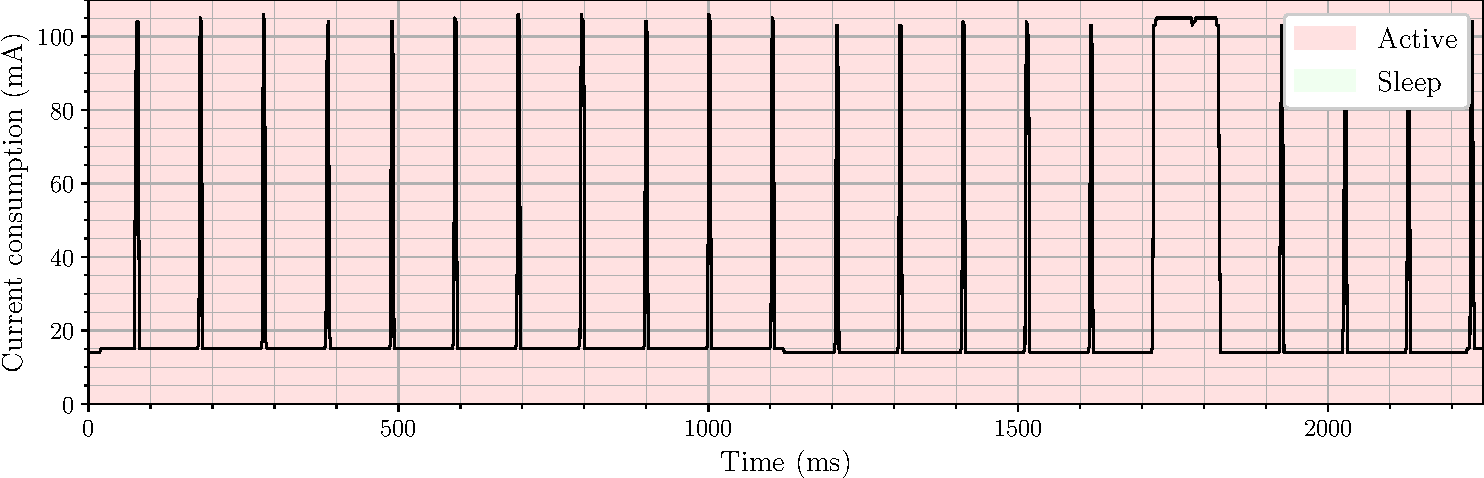
\includegraphics[width=\textwidth]{blink-old-plot.pdf}
	\end{minipage}
	\begin{minipage}{0.9\textwidth}
		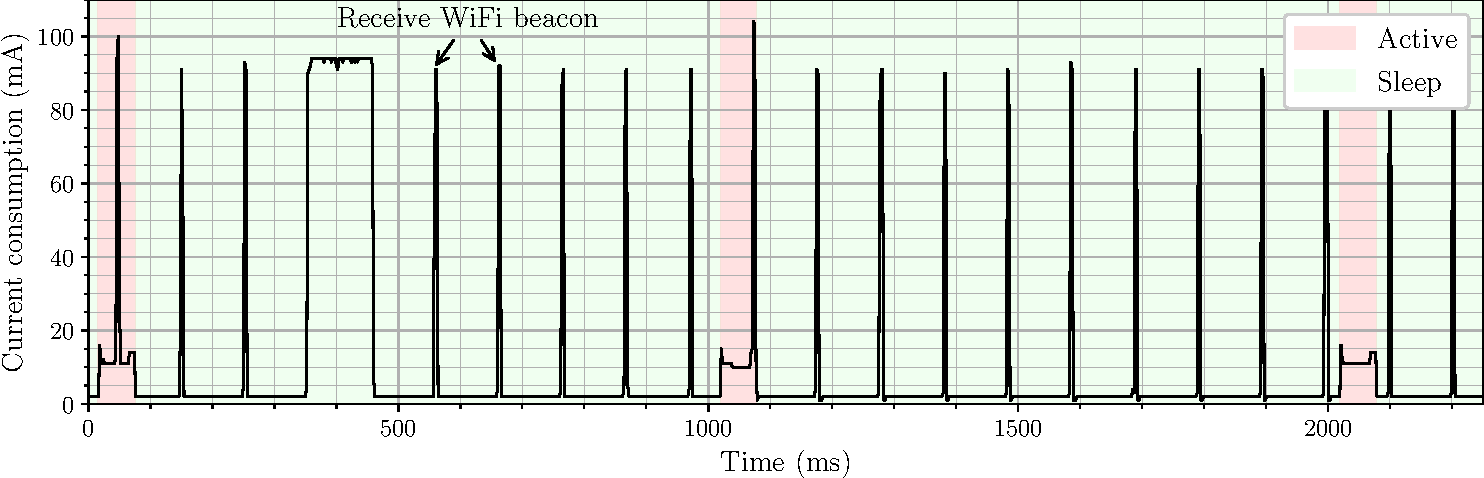
\includegraphics[width=\textwidth]{blink-plot.pdf}
	\end{minipage}
	\caption{Current draw of the blink task with the old implementation on top.}%
	\label{fig:blink_current}
%	\vspace{-1cm}
\end{figure}

\paragraph{Thermometer Example}

The thermometer task just reads the temperature from a Wemos SHT30 sensor%
\footnote{See \url{https://www.wemos.cc/en/latest/d1_mini_shield/sht30.html}}.

\begin{lstlisting}[language=Clean,caption={A basic thermometer task.},label={lst:thermometer}]
thermometer :: Main (MTask v Bool) | mtask v
thermometer = DHT I2Caddr \sensor.
              {main = temperature` (BeforeSec (lit 60)) sensor}
\end{lstlisting}

The measurement will be repeated since this produces an unstable value.
Figure~\ref{fig:temp_current} depicts the current consumption of this example.
The longer upper bound of the refresh interval enables deep sleep between individual measurements.
As a consequence, the Wi-Fi connection needs to be re-established after waking up, resulting in a longer current spike.

\begin{figure}[ht]
	\centering
	\begin{minipage}{0.9\textwidth}
		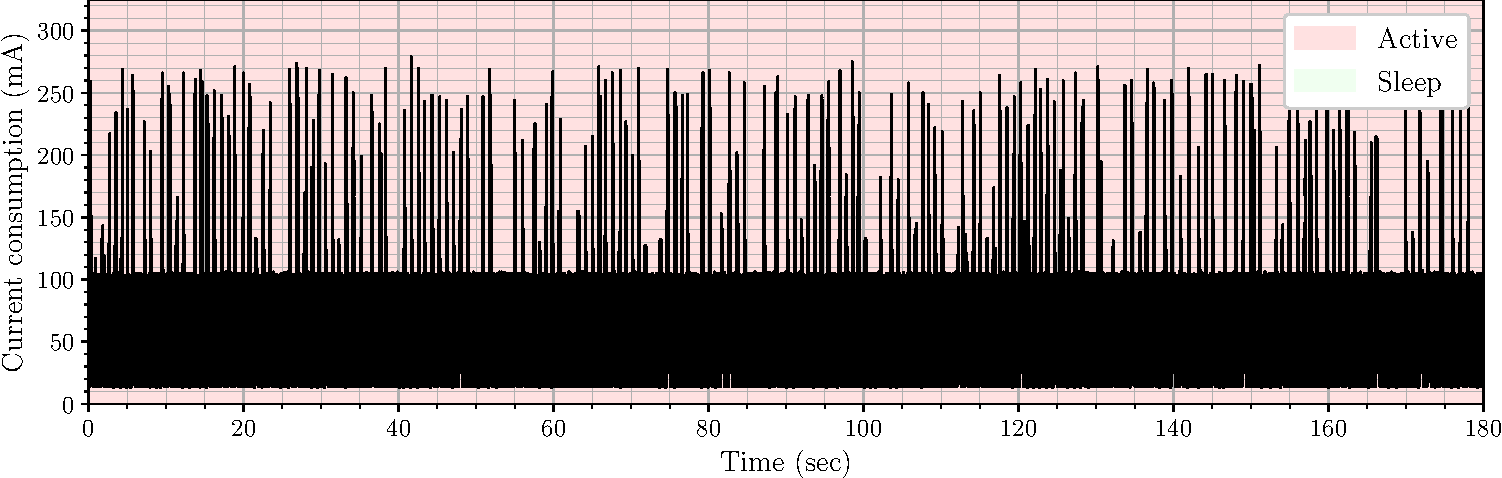
\includegraphics[width=\textwidth]{temp-old-plot.pdf}
	\end{minipage}
	\begin{minipage}{0.9\textwidth}
		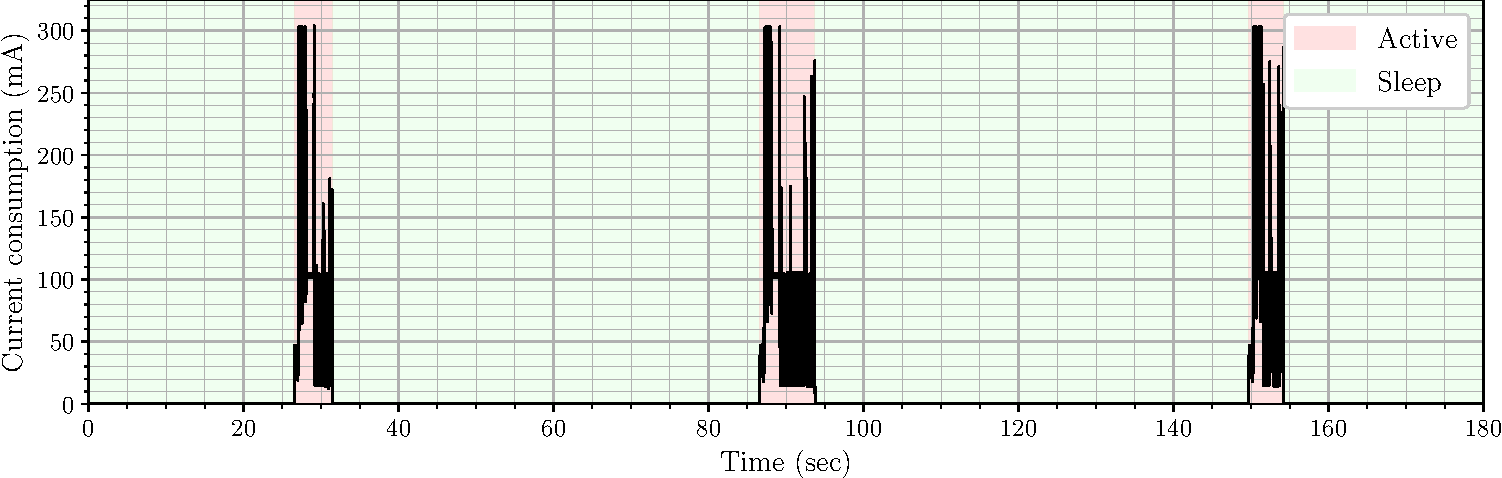
\includegraphics[width=\textwidth]{temp-plot.pdf}
	\end{minipage}
	\caption{Current draw of the temperature task with the old implementation on top.}%
	\label{fig:temp_current}
%	\vspace{-.5cm}
\end{figure}

\paragraph{PIR Switch Example}

Next, we consider the PIR switch example from Listing~\ref{lst:pirSwitch}.
Since the old version of mTask does not support interrupts, we cannot execute the program directly.
To mimic the effect as well as possible, we replaced \prog{interrupt High pirPin} by a polling solution that waits until the pin reading is high; \prog{readD pirPin >>*. [IfValue id rtrn]}.
The measurement results are similar to the previous example, constant activity in the old implementation and sleep with small bursts in the new implementation.
The actual interrupts determine the number of bursts seen so it does not make sense to plot the current.
%\mlcomment{No figure here}
%\pkcomment{Klopt. Is er niet en ik probeer uit te leggen dat die ok niet erg nuttig is.}
%\mlcomment{Ik heb het uitgebreid zodat het hopelijk duidelijker is waarom er geen plaatje is}

% \begin{lstlisting}[language=Clean,caption={Two versions of the light switch.},label={lst:lightswitch}]
% lightSwitchOld :: Main (MTask v Bool) | mtask v
% lightSwitchOld
%   = declarePin ButtonPin PMInput \button ->
%     declarePin BuiltinLEDPin PMOutput \led ->
%       fun \switch=(\x->
%         writeD led x
%         >>|. delay (lit 50)             // Debounce
%         >>|. readD button               // Poll until button pressed
%         >>*. [IfValue Not (\_.switch (Not x))])
%     In {main=switch (lit False)}

% lightSwitch :: Main (MTask v Bool) | mtask v
% lightSwitch
%   = declarePin ButtonPin PMInput \button ->
%     declarePin BuiltinLEDPin PMOutput \led ->
%       fun \switch=(\x->
%         writeD led x
%         >>|. delay (lit 50)             // Debounce
%         >>|. interrupt Falling button   // wait for interrupt
%         >>|. switch (Not x))
%     In {main=switch false}
% \end{lstlisting}

\paragraph{Plant Monitor}

This task observes a plant's environment and monitors two values, the amount of water in the soil and the light intensity.
It becomes stable when one of the monitored values exceeds a threshold.
The value of the soil sensor should be read at least every 5 minutes, 300 seconds, and the light intensity at least every 90 seconds.

\begin{lstlisting}[language=Clean,caption={The plant monitor task.},label={lst:plantMonitor}]
monitorPlant :: Main (MTask v Bool) | mtask, dht, LightSensor v
monitorPlant = {main = lightSensor .||. moistureSensor}
where
    moistureSensor = readA` (BeforeSec (lit 300)) MoistureSensorPin
                   >>*. [IfValue ((<=.) moistureThreshold) (\_. rtrn true)]
    lightSensor    = light` (BeforeSec (lit 90)) lightsensor
                   >>*. [IfValue ((<=.) lightThreshold) (\_. rtrn true)]
\end{lstlisting}
The combined refresh rate of the combinator \prog{.||.} is determined by the shortest interval: $\langle 0, 90 \times 1000 \rangle$.
We execute this task and the thermometer from Listing~\ref{lst:thermometer} on the same node.
The thermometer task has a refresh interval of $\langle 0, 60 \times 1000 \rangle$.
Hence, we should see the execution of both tasks every 60 seconds.
This is exactly what is shown in Figure~\ref{fig:complex}.

\begin{figure}[ht]
	\centering
	\begin{minipage}{0.9\textwidth}
		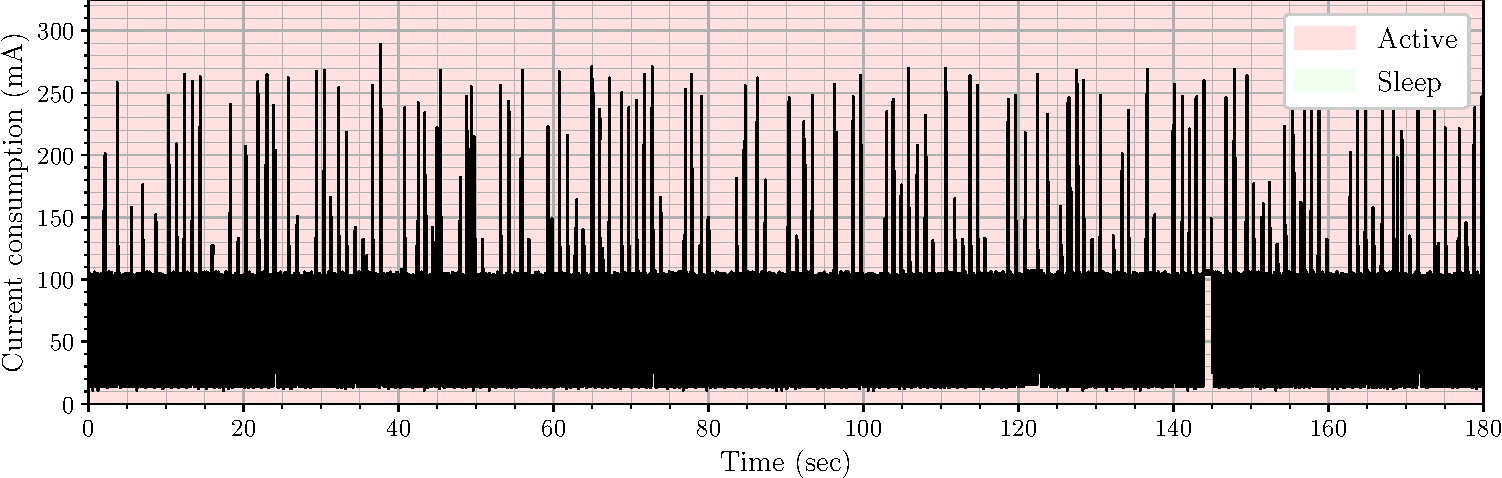
\includegraphics[width=\textwidth]{complex-old-plot.pdf}
	\end{minipage}
	\begin{minipage}{0.9\textwidth}
		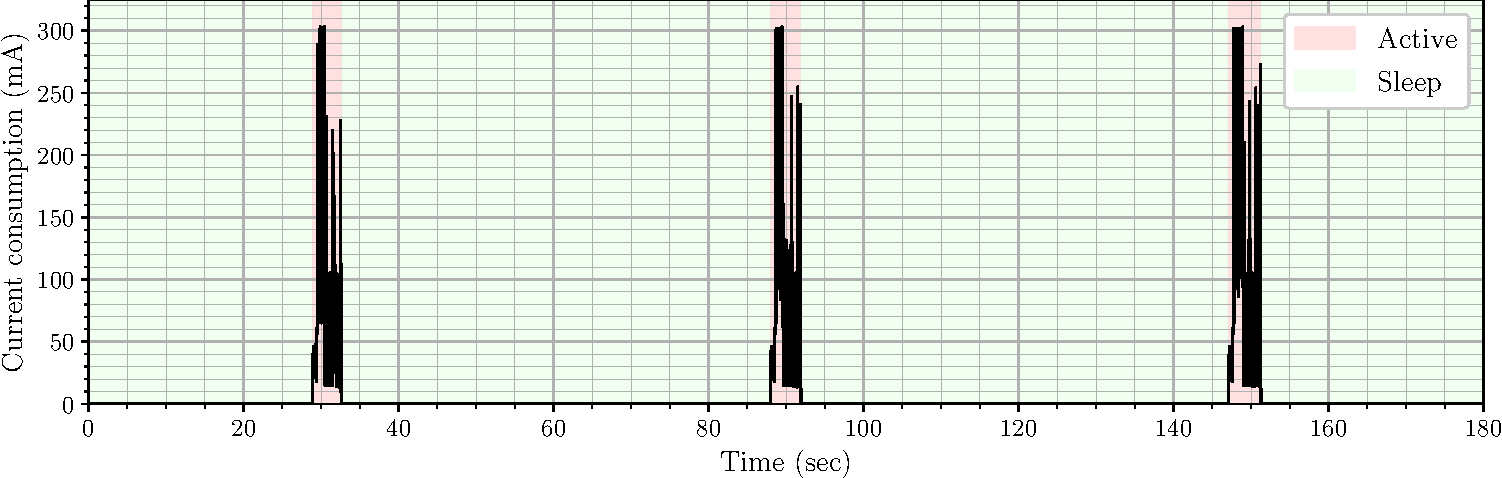
\includegraphics[width=\textwidth]{complex-plot.pdf}
	\end{minipage}
	\caption{Current draw of the thermometer task and the plant monitor.}%
	\label{fig:complex}
%	\vspace{-.2cm}
\end{figure}

\subsection{Power Saving}

By integrating with the composite trapezoidal rule, we calculate the total power consumption from the shown current measurements.
The number of interrupts determines the saving for the PIR sensor example.
Hence, we have not included these numbers in the table.
Table~\ref{tab:energy} shows that our implementation works as expected.
It reduces the energy consumption in all our examples considerably.

\begin{table}[ht]
	\centering
	\begin{tabular}{lccc}
		\toprule
		Task        & \multicolumn{2}{l}{Average energy consumption} & Difference \\
					& Old                    & New  &             \\
					\midrule

		Blink       & 111.3 mW               & 52.1 mW &   -53\%            \\
		Thermometer & 204.2 mW               & 28.8 mW &
		-86\%\\

		Combined & 190.2 mW               & 22.5 mW    & -88\%  \\
		\bottomrule
	\end{tabular}
	\caption{Energy consumption and saving of the example programs.}%
	\label{tab:energy}
%	\vspace{-1cm}
\end{table}

\section{Related Work}

Reducing the energy consumption of IoT nodes is currently getting attention from several directions.
More modern microprocessors are typically bigger in terms of memory and computation power, while they consume less energy.
Our work is complementary to this approach.

\subsubsection{Task-Oriented Programming}

Most implementation work for TOP is part of the iTask system~\cite{TOP-ICFP07,TOP-PPDP12}.
The iTask framework generates web servers running on a normal computer.
The efficiency of the generated programs focusses on short response times and preventing unnecessary computations.
It also implements a sophisticated publish-subscribe system to handle updates caused by {SDS}.
It is worthwhile to investigate if such a system can be implemented within the context of a microprocessor based system.

\subsubsection{Functional Reactive Programming}

Implementations of functional reactive programming (FRP) for microprocessors have similar goals as the mTask implementation of TOP~\cite{ElliottHudak97:Fran}.
The TOP system approaches the program from the tasks to be done and the change of those tasks.
The FRP approach approaches the program from the streams of data from sensors and other inputs.
This results in quite different programming styles~\cite{frp_vs_top}.

Hae is a DSL for FRP deeply embedded in Haskell that generates C++ code.
This code will be loaded in the flash memory of the microprocessors~\cite{Hae}.
Hence, it cannot be updated as often and easy as the task in our mTask system.

Belwal et al.\ present an energy reduction technique for FRP based on Dynamic Voltage and Frequency Scaling (DVFS)~\cite{dvfs_frp}. Instead of bringing the system to sleep, they reduce the energy consumption by slowing the processor down.

\subsubsection{Embedded DSLs for Programming Microprocessorsrs}

There are some other DSLs for programming microprocessors embedded in Functional Programming Languages.
Haskino comes in various variants~\cite{Haskino}.
It enables to dynamically execute abstractions of Arduino statements on a small microprocessor.
Haski focuses on the secure communication with IoT nodes~\cite{Haski}.

\subsubsection{Embedded Operating Systems}

There are several embedded operating systems geared towards microprocessors, like FreeRTOS~\cite{FreeRTOS}, Mantis OS~\cite{Mantis} and Nano RK~\cite{Nano_rk}.
Those systems offer pre-emptive multitasking on microprocessors as well as several ways to reduce energy consumption.
In contrast to the mTask system, those systems store the programs in flash memory and are hence less dynamically.
Moreover, they are based on C-programs and cannot offer the reflection on the current state of tasks.
Sleep modes must typically be invoked explicitly in the user program, or are at best invoked when all threads in the program explicitly invoke a sufficient long delay.

\section{Conclusion}

In this paper, we show how we can automatically associate execution intervals to tasks.
Based on these intervals, we can delay the executions of those tasks.
When all task executions can be delayed, the microprocessor executing those tasks can go to sleep mode to reduce its energy consumption.
This is a rather difficult problem that must be solved dynamically, since we make no assumptions on the number and nature of the tasks that will be allocated to an IoT node.
Furthermore, the execution intervals offer an elegant and efficient way to add interrupts to the language.
Those interrupts offer a more elegant and energy efficient implementation of watching an input than polling this input.

The actual reduction of the energy is of course highly dependent on the number and nature of the task shipped to the IoT node.
Our examples show a reduction in energy consumption of two orders of magnitude.
Those reductions are a necessity  for IoT nodes with battery power.
Given the exploding number of IoT nodes, such savings are also mandatory for other nodes to limit the total power consumption of the IoT.
%\mlcomment{Hier moet ook nog iets over interrupts denk ik}

\section*{Acknowledgements}\label{sec:acknowledgments}
This research is partly funded by the Royal Netherlands Navy.
Furthermore, we would like to thank the anonymous reviewers for their invaluable comments.

%
% ---- Bibliography ----
%
% BibTeX users should specify bibliography style 'splncs04'.
% References will then be sorted and formatted in the correct style.
%
\bibliographystyle{splncs04}
\bibliography{bibliography}
%
\end{document}
